\documentclass[onecolumn,10pt]{article}
\linespread{1.3}
\usepackage[margin=2cm]{geometry}

\usepackage[utf8]{inputenc}
\usepackage[spanish]{babel}
\usepackage{tikz}
\usepackage{paralist}
\usepackage{subcaption} \usepackage{graphicx}
\usepackage{amsmath} \usepackage{amssymb}
\usepackage{xcolor}
\usepackage{listings}

\usepackage{amsmath}
\usepackage{algorithm}
\usepackage[noend]{algpseudocode}

\lstset{language=C}
\bibliographystyle{apsrev4-1}

\graphicspath{{./fig/}}

\newcommand{\IDT}{\texttt{IDT}}
\newcommand{\MMU}{\texttt{MMU}}
\newcommand{\GDT}{\texttt{GDT}}
\newcommand{\TSS}{\texttt{TSS}}
\newcommand{\PD}{\texttt{PD}}

\begin{document} 

\title{Trabajo Práctico 1: Redes Neuronales Artificiales}

\author{L. Alvarez, P. Bordon y D. Santos}

\date{\today}

%\begin{abstract}
%\end{abstract}

\maketitle


\newpage

\tableofcontents

\newpage

\section{Ejercicio 1: Clasificación de Resultados de Diágnostico de Cancer de Mama utilizando Perceptron Multicapa}

\subsection{Introducción}
La primer etapa del trabajo practico consiste en la implementación
de una red neuronal para la clasificación de diagnostico de cancer
de mama a partir de un dataset con los resultados de analisis y
su diagnostico clasificados en \textbf{B} (benigno) o \textbf{M} (maligno).

El objetivo es determinar si es posible aplicar \emph{Redes Neuronales} para
diagnosticar de forma efectiva si un tumor es \textbf{Benigno} o \textbf{Maligno}.

Para lograr el objetivo presentaremos una \emph{Red Neuronal} basada en la
implementación de un \textbf{Perceptron Multicapa}.

Para dicha implementación las etapas desarrolladas son:

\begin{itemize}
\item Análisis de la Red: Describiremos los primeros enfoques a la
  solución propuesta
\item Prepocesamiento de datos: Proceso aplicado al dataset recibido.
\item Arquitectura definitiva: Implementación final de la arquitectura
  de la red.
\item Implementación de la Red: La implementación del perceptron y sus
   algoritmos.
\end{itemize}


\subsection{Análisis de la Red}

La primera aproximación a la solucion fue implementar una red de una
capa con 8 neuronas, la cantidad de neuronas elegida fue alta, 
entendiendo que podía generarnos el problema de \emph{overfitting}.
Siendo nuestro objetivo principal estudiar el aprendizaje de la red
para luego ir ajustando la cantidad de capas y neuronas.
Como función de activación elegimos la tangente hiperbólica. 
Contrario a lo esperado, nuestra primera red no lograba \emph{aprender}.
Obteníamos un \emph{Error Cuadrático Medio} alto en promedio. Y a pesar
de incrementar la cantidad de iteraciones se estancaba en valores
cercanos al 0.50 aproximadamente, haciendo imposible una correcta
clasificación.
Lo siguiente fue empezar a modificar la arquitectura de la red,
variando la cantidad de neuronas y al seguir sin mejoras, agregamos
sin éxito una segunda capa de neuronas.

Descubrimos que el motivo por el cual la red se comportaba de esta
forma se debía a que al aplicar la función de activación a los valores
del dataset estos alcanzaban el valor 1 siempre. Entonces para corregir
el problema realizamos un pre-procesamiento de los datos.


\subsection{Procesamiento de Datos}

Para solucionar el problema que genera aplicarle la función de activación
al dataset realizamos un pre procesamiento de los datos.
Este procesamiento consiste en \emph{normalizar} los datos con varianza = 0 y
sigma = 1.

Con este procesamiento nos aseguramos que aplicandole la función de
activación de tangente hiperbólica a los datos obtenemos valores entre
0 y 1.

\subsection{Arquitectura definitiva}

Con los datos procesados comenzamos con las pruebas para encontrar
una arquitectura lo suficientemente robusta para alcanzar un buen nivel
de aprendizaje pero que no caiga en la redundancia del \emph{overfitting}.

Implementamos una arquitectura de una sola capa interna, con 10 + 1 neuronas 
en la capa de entrada, 10 para los datos del data set y una inicializada en -1
y 1 neurona en la de salida. Para la capa interna implementamos
soluciones con distinta cantidad de neuronas en la segunda capa, tomando 
valores de 8 a 5 y realizamos pruebas variando los parametros de
 \emph{leanrning rate}, \emph{cantidad de iteraciones} y \emph{tolerancia de error}.

 Mas adelante presentaremos los resultados obtenidos en la sección de \textbf{Resultados}

 Luego de realizar los experimentos detectamos que la arquitectura que presenta
 mejor adaptación para el aprendisaje es la que implementa una capa interna de entre
 5 o 6 neuronas.

 Entonces la arquitectura definitiva propuesta es:

10 + 1 neuronas como \emph{entrada}, una capa \emph{interna} de 5 neuronas 
y 1 neurona para la capa de \emph{salida}.

Para entrenar la red lo hacemos con el 80 por ciento de los datos del dataset,
el resto los dejamos para validación.

Definimos una función de activación basada en la tangente hiperbólica para ambas
capas, pero dejamos la libertad de utilizar distintos parametros de beta en cada
una de ellas.

Una vez entrenada la red corremos un algoritmo de testoe basado en la técnica de
\textbf{cross-validation}.

El parametro \textbf{cantidad-mezclas} es el que define la cantidad de veces que
el algoritmo toma \emph{k-folds} del dataset para entrenar y validar.


\subsection{Implementación de la Red}

A continuación detallaremos como implementamos la red.

Implementamos una clase \textbf{Perceptron} con la siguiente estructura

\begin{lstlisting}
  struct perceptron {
    learning_rate 
    beta1 
    beta2
    tolerancia_error
    cantidad_repeticiones
    cantidad_mezclas
    input_file 
    output_file
    tamano_capa
    tamano_entrada
    tamano_salida 
    w1  
    w2  
  }

\end{lstlisting}


\begin{itemize}
\item \textbf{learning rate} = coeficiente de aprendizaje.
\item \textbf{beta1} = parametro beta en la primera función de activación.
\item \textbf{beta2} = parametro beta en la segunda función de activación.
\item \textbf{tolerancia-error} = tolerancia de error.
\item \textbf{cantidad repeticiones} = cantidad de epocas.
\item \textbf{cantidad mezclas} = cantidad de veces que se ejecutará.
\item \textbf{input file} = archivo de entrada.
\item \textbf{output file} = archivo de salida.
\item \textbf{tamano capa} = tamaño de capa interna.
\item \textbf{tamano entrada} = tamaño de capa de entrada.
\item \textbf{tamano salida} = tamaño de capa de salida.
\item \textbf{w1} = vector de pesos de la primer capa.
\item \textbf{w2} = vector de pesos de la segunda capa.
\end{itemize}


Definida la estructura principal del \textbf{Perceptron} presentamos
las funciones principales que utilizá la \emph{Red Neuronal} para
la clasificación de datos.


\begin{itemize}
\item \textbf{entrenar} = entreniento de la red, realiza el preprocesamiento
del dataset, y para la cantidad seteada de mezclas realiza un entrenamiento, tomando
como cota la cantidad de iteraciones y la tolerancia del error. Dentro del ciclo principal
calcula la activación, corrección y adaptación de la red. Luego realiza cross-validation para
verificar los resultados de cada época.
\item \textbf{testing} = toma una red entrenada y calcula la tasa de aciertos.
\item \textbf{funcion activacion} = funcion de activación.
\item \textbf{funcion activacion derivada} = funcion de activación derivada.
\end{itemize}


\subsection{Experimentación y Resultados}



Definida la red procedemos a realizar  un entrenamiento de la misma 
variando el tamaño de la capa interna, entrenamos el suficiente tiempo para
encontrar el punto donde empieza a converger el ECM.

La primera configuración es la siguiente

\begin{itemize}
\item \textbf{learning-rate} = 0.1
\item \textbf{beta1} = 0.1
\item \textbf{beta2} = 0.1
\item \textbf{tolerancia-error} = 1.
\item \textbf{cantidad-repeticiones} = 10000.
\item \textbf{cantidad-mezclas} = 10.
\item \textbf{tamano-capa} = 5.
\end{itemize}


Tomamos la salida con menor ECM y presentamos en un gráfico la convergencia
de los errores:

\begin{figure}[H]
  \centering
  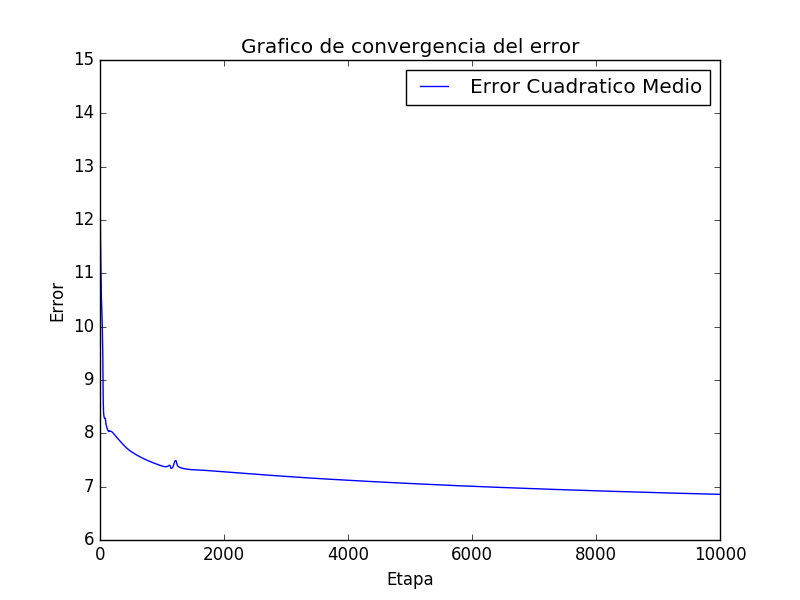
\includegraphics[width=0.8\columnwidth]{red_5_ecm.png}
  \caption{Comparación contra ECM.}
  \label{fig:red 5 ECM}
\end{figure}



%\begin{figure}[H]
%  \centering
%   \includegraphics[width=0.8\columnwidth]{red_5_prom.png}
%  \caption{Comparación mínimo, promedio y máximo.}
%  \label{fig:red promedios}
%\end{figure}

Podemos observar que el ECM durante las primeras 2000 iteraciones fue descendiendo
y a partir de la iteracion 2000 el descenso fue menor, pero siempre en baja.
No alcanzamos un punto donde empieze a oscilar.

La comparativa de los errores Promedio, Mínimo y Máximo muestra que se mantuvieron
casi constante y no variaron a pesar de las 10000 iteraciones.

Procedemos a ejecutar la función test para ver que resultados produjo el entrenamiento 

La tasa de aciertos luego de ejecutar la función testing se úbico 367 en sobre 410.

Adjuntamos la red entrenada en el archivo: red-5-train.in.



Repetimos el mismo experimento para una red de 6 neuronas:

\begin{itemize}
\item \textbf{learning-rate} = 0.1
\item \textbf{beta1} = 0.1
\item \textbf{beta2} = 0.1
\item \textbf{tolerancia-error} = 1.
\item \textbf{cantidad-repeticiones} = 10000.
\item \textbf{cantidad-mezclas} = 10.
\item \textbf{tamano-capa} = 6.
\end{itemize}


Presentamos los resultados correspondientes a la mezcla que produjo
el menor ECM:

\begin{figure}[H]
  \centering
  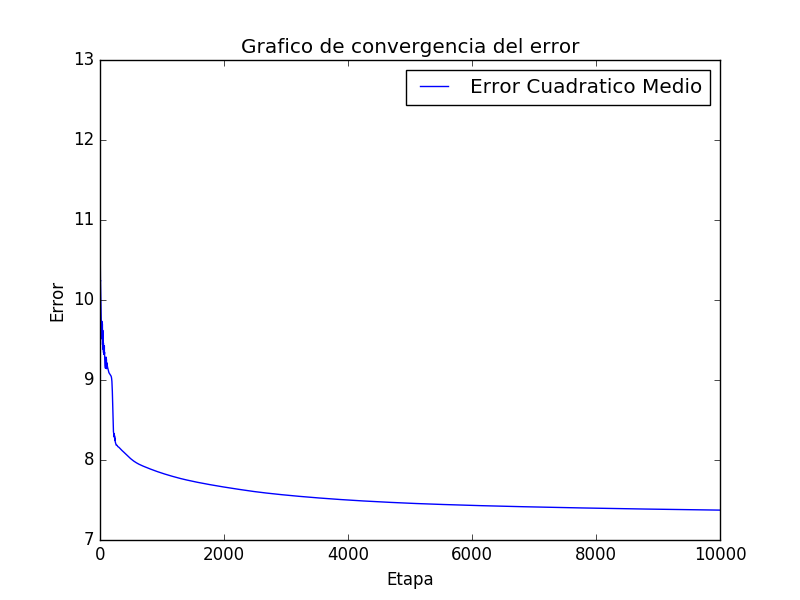
\includegraphics[width=0.8\columnwidth]{red_6_ecm.png}
  \caption{Comparación contra ECM.}
  \label{fig:red 6 ECM}
\end{figure}


\begin{figure}[H]
  \centering
  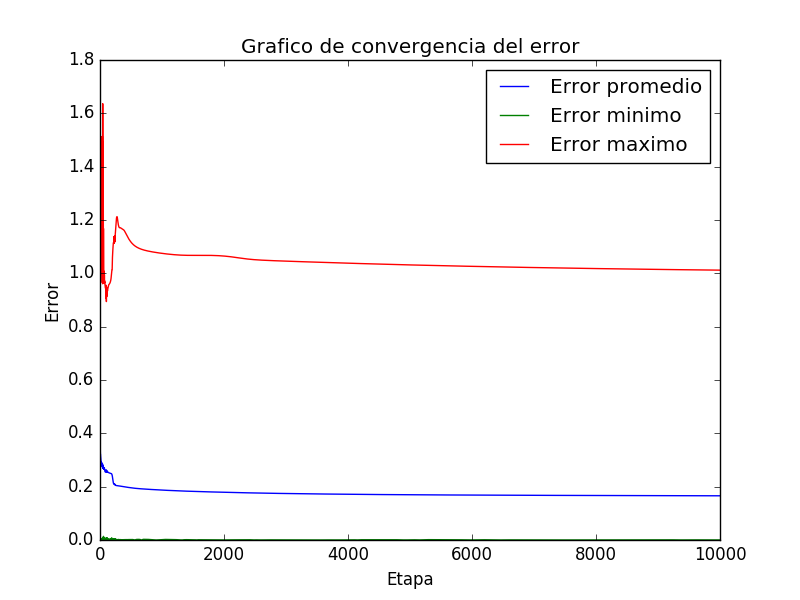
\includegraphics[width=0.8\columnwidth]{red_6_prom.png}
  \caption{Comparación mínimo, promedio y máximo.}
  \label{fig:red promedios}
\end{figure}

La comparativa nos muetsra que el error Máximo oscila mucho en las primeras 
iteraciones y luego se estabiliza y se mantiene constante.

El ECM promedio fue de 7.008, es decir relativamente superior al menor de la red
de 5 neuronas en la capa interna. De nuevo vemos que a partir de la iteración 2000
comienza a descender muy lentamente.

La tasa de aciertos luego de ejecutar la función testing se úbico en 370 sobre 410.
Siendo apenas superior por a la red de 5 neuronas, esto se reduce a esta instancia 
particular no hay garantía de que siempre sea mejor.


Adjuntamos la red entrenada en el archivo: red-6-train.in.

Ahora realizamos el mismo experimento para una red de 4 neuronas:

\begin{itemize}
\item \textbf{learning-rate} = 0.1
\item \textbf{beta1} = 0.1
\item \textbf{beta2} = 0.1
\item \textbf{tolerancia-error} = 1.
\item \textbf{cantidad-repeticiones} = 10000.
\item \textbf{cantidad-mezclas} = 10.
\item \textbf{tamano-capa} = 4.
\end{itemize}


Presentamos los resultados correspondientes a la mezcla que produjo
el menor ECM:

\begin{figure}[H]
  \centering
  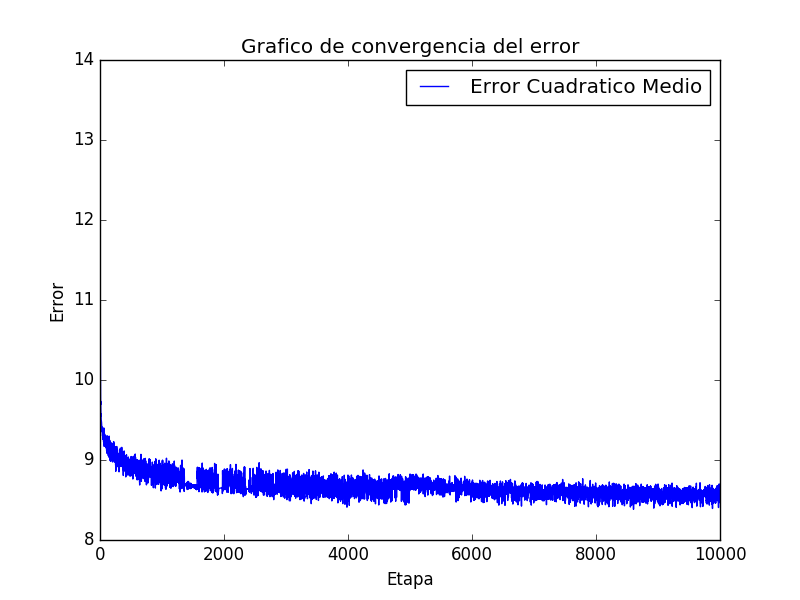
\includegraphics[width=0.7\columnwidth]{red_4_ecm.png}
  \caption{Comparación contra ECM.}
  \label{fig:red 4 ECM}
\end{figure}


\begin{figure}[H]
  \centering
  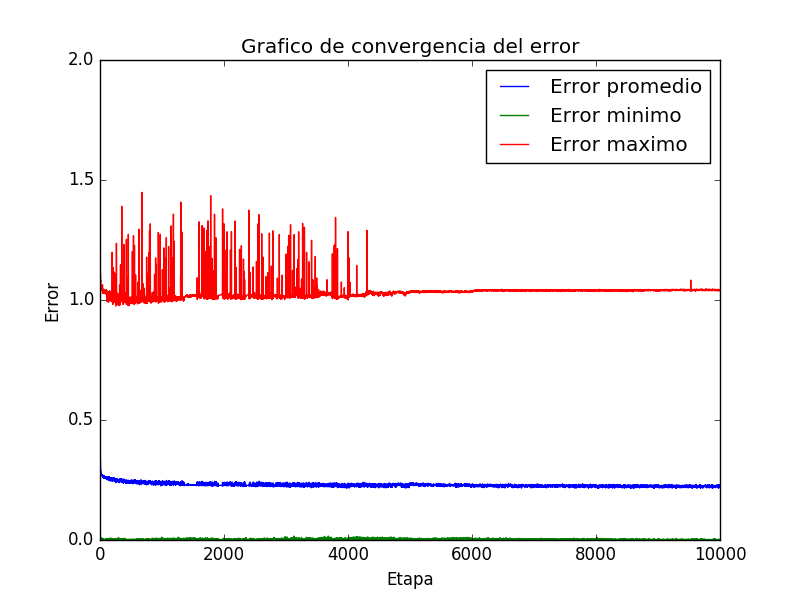
\includegraphics[width=0.7\columnwidth]{red_4_prom.png}
  \caption{Comparación mínimo, promedio y máximo.}
  \label{fig:red promedios}
\end{figure}

El ECM promedio que se obtuvo fue de 8,67 muy superior a las otras redes, además se
puede notar que el ECM oscila mucho entre las iteraciones, es decir no siempre desciende.

En la comparativa de los errores se puede ver que al máximo le lleva muchas iteraciones
estabilizarse, aunque no lo logra del todo. El promedio y el mínimo tambiém se mantienen
oscilantes

La tasa de aciertos luego de ejecutar la función testing se úbico en 355 sobre 410.

Damos por descartado que la red con una capa interna de 4 neuronas sea la mejor opción.
De todas formas adjuntamos la red en el archivo red-4-train.in

De los experimentos realizados la red con 5 neuronas fue la que a priori puede brindar
mejores resultados es la que tiene 5 neuronas en la capa interna. Nos resulto ser una red lo suficientemente robusta para aprender sin caer en el riesgo de \emph{overfitting}.

Vamos a estudiar que tan bien responde con instancias mas cortas de entrenamiento. Ahora vamos
entrenar la red con los siguientes parámetros:

\begin{itemize}
\item \textbf{learning-rate} = 0.1
\item \textbf{beta1} = 0.1
\item \textbf{beta2} = 0.1
\item \textbf{tolerancia-error} = 1.
\item \textbf{cantidad-repeticiones} = 500.
\item \textbf{cantidad-mezclas} = 5.
\item \textbf{tamano-capa} = 5.
\end{itemize}

El objetivo es ver si con menos instancia de entrenamiento adquiere una proporción
similar de resultados.

Presentamos los resultados correspondientes a la mezcla que produjo
el menor ECM:


\begin{figure}[H]
  \centering
  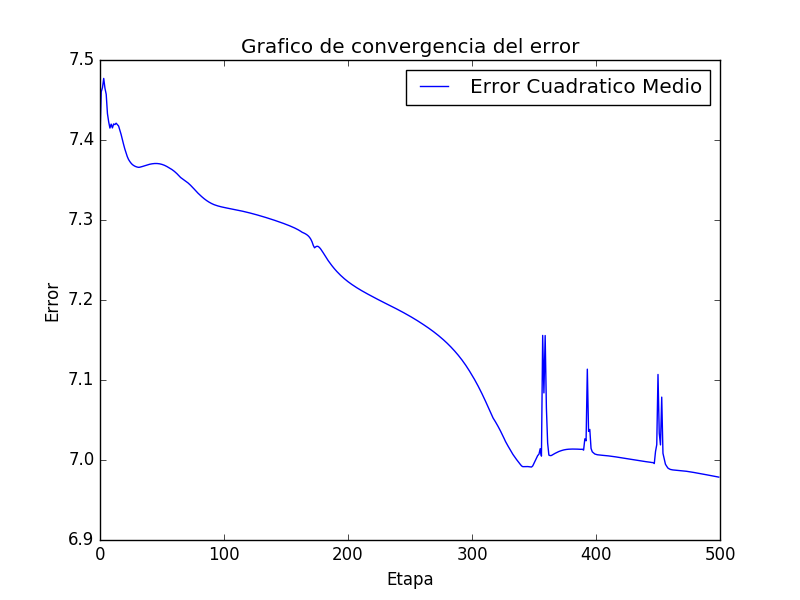
\includegraphics[width=0.7\columnwidth]{red_5_ecm_reducida.png}
  \caption{Comparación contra ECM.}
  \label{fig:red 5 ECM}
\end{figure}


\begin{figure}[H]
  \centering
  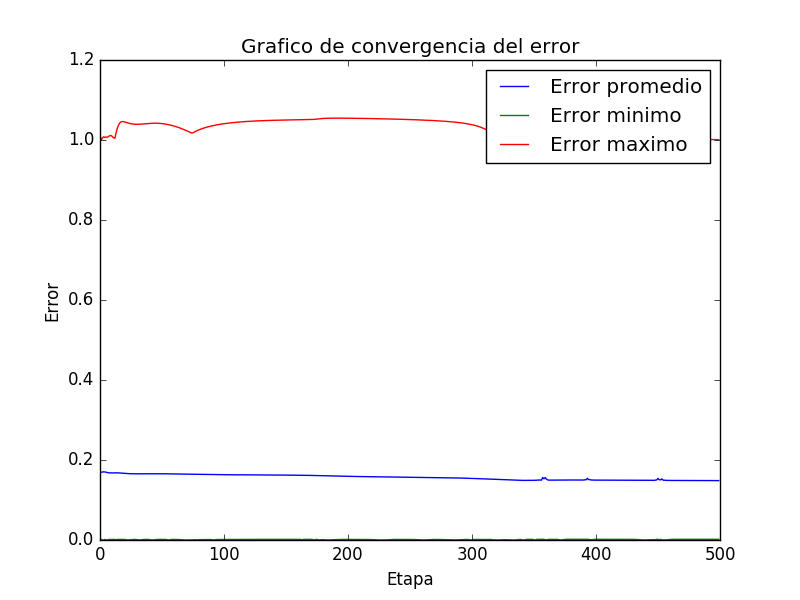
\includegraphics[width=0.7\columnwidth]{red_5_prom_reducida.png}
  \caption{Comparación mínimo, promedio y máximo.}
  \label{fig:red promedios}
\end{figure}

El ECM promedio se ubico en 6.97

Vemos que los graficos de errores se acomodan rapidamente tendiendo a valores obtenidos
con mas iteraciones-

La tasa de aciertos luego de ejecutar la función testing se úbico en 387 sobre 410.

Repetimos el experimento varias veces y en todos los casos obtuvimos aciertos entre los
382-397, nos hace pensar que entrenar con iteraciones de mas no siempre es lo mejor.
Ya que podriamos estas sobreentrenando la red, causando que esta memorize los valores
y pierda el sentido de la predicción.

Adjuntamos la red en el archivo red-5-train-reducida.in


\subsection{Concluciones}

La \textbf{Red Neuronal} propuesta basada en una implementación del Perceptrón Multicapa,
logro en gran parte de las ejecuciones un alto porcentaje de aciertos, sobre todo a 
partir del último experimento.
Esta técnica puede ser util para ayudar en el diagnostico del cancer de mama, pero
no debe ser la única aplicada. Ya que la información y el veredicto inciden
sobre la vida de la persona diagnosticada, seria prudente cotejar los resultados
con técnicas mas sofisticadas de dianóstico.


\newpage


\section{Ejercicio 2: Modelos MLP aplicados al análisis de eficiencia energética en edificios}


\subsection{Introducción}

El objetivo en este caso consistió en predecir el valor de carga energética necesaria para la calefacción y refrigeración de edificios a partir de ciertas características de los mismos. El conjunto de datos contaba con valores sobre 8 características distintas a tener en cuenta y se debió entrenar al sistema a partir de 500 resultados dados tanto para calefacción como para refrigeración.   



\subsection{Análisis de la red}

En primera instancia utilizamos una arquitectura similar a la implementada en la primera parte del trabajo. Una capa de entrada de 8 + 1 neuronas, una única capa oculta de número de neuronas variables entre 5 y 8, función de activación sigmoide de tipo bipolar (tanh($\beta$X)) y en este caso 2 neuronas en la capa de salida de salida, una para la carga de refrigeración y otra para la carga de calefacción. Contrario a lo que esperábamos la red no lograba aprender, obteniendo valores de salida para las cargas de refrigeración y calentamiento poco correlacionados con los de los datos de entrenamiento, no logrando bajar el error de entrenamiento. Debido a esto, lo siguiente fue empezar a cambiar la arquitectura de la red, variando los parámetros de activación, taza de aprendizaje y número de neuronas, sin obtener mejoras significativas.
Pasamos a cambiar la función de activación, optando por una lineal  (f(X)=x), ya que la función sigmoidal nos acotaba los valores, mientras que los resultados esperados estaban entre 5 y 20.


\subsection{Procesamiento de datos}

De manera análoga al caso anterior, en vista de que las medias y varianzas de unos y otros atributos difieren significativamente y hacen que ciertos dominen en detrimento de otros, pasamos a normalizar los datos para uniformarlos. De esta forma los atributos normalizados tienen media cero y varianza 1, moviéndose en un rango de valores similar. A los datos asociados a las cargas de refrigeración y calefacciones no se les aplicó la normalización.


\subsection{Arquitectura de la red}

Con los datos preprocesados y fijando una función de activación lineal, comenzamos con las pruebas para obtener una arquitectura óptima, variando el número de capas, taza de aprendizaje, cantidad de iteraciones y tolerancia del error
Luego de realizar los experimentos detectamos que la arquitectura que presenta mejor adaptacion al aprendizaje es xxxxxx

De esta forma, la arquitectura definitiva propuesta consiste en una capa de entrada de 8 + 1 neuronas, capa oculta de xxx neuronas y capa de salida de dos neuronas.  Al igual que en el caso anterior, el entrenamiento lo hacemos con el 80% del dataset, dejando los restantes para validar. 


\subsection{Implementación de la red}

A continuación detallaremos como implementamos la red.


Implementamos una clase \textbf{Perceptron} con la siguiente estructura

\begin{lstlisting}
  struct perceptron {
    learning_rate 
    tolerancia_error
    cantidad_repeticiones
    cantidad_mezclas
    input_file 
    output_file
    tamano_capa
    tamano_entrada
    tamano_salida 
    w1  
    w2  
  }

\end{lstlisting}


\begin{itemize}
\item \textbf{learning rate} = coeficiente de aprendizaje.
\item \textbf{tolerancia-error} = tolerancia de error.
\item \textbf{cantidad repeticiones} = cantidad de epocas.
\item \textbf{cantidad mezclas} = cantidad de veces que se ejecutará.
\item \textbf{input file} = archivo de entrada.
\item \textbf{output file} = archivo de salida.
\item \textbf{tamano capa} = tamaño de capa interna.
\item \textbf{tamano entrada} = tamaño de capa de entrada.
\item \textbf{tamano salida} = tamaño de capa de salida.
\item \textbf{w1} = vector de pesos de la primer capa.
\item \textbf{w2} = vector de pesos de la segunda capa.
\end{itemize}


Definida la estructura principal del \textbf{Perceptron} presentamos
las funciones principales que utilizá la \emph{Red Neuronal} para
la clasificación de datos.


\begin{itemize}
\item \textbf{entrenar} = entreniento de la red, realiza el preprocesamiento
del dataset, y para la cantidad seteada de mezclas realiza un entrenamiento, tomando
como cota la cantidad de iteraciones y la tolerancia del error. Dentro del ciclo principal
calcula la activación, corrección y adaptación de la red. Luego realiza cross-validation para
verificar los resultados de cada época.
\item \textbf{testing} = toma una red entrenada y calcula la tasa de aciertos.
\item \textbf{funcion activacion} = funcion de activación.
\item \textbf{funcion activacion derivada} = funcion de activación derivada.
\end{itemize}


\subsection{Experimentación y resultados}

Definida la red procedemos a realizar un entrenamiento de la misma variando el tamaño de la capa interna, entrenamos el suficiente tiempo para encontrar el punto donde empieza a converger el ecm.


En la primer corrida obtenemos un ECM promedio de 3.74369233105. Los gráficos \ref{fig:ej2_c1_train0} y \ref{fig:ej2_c1_train1} representan el error promedio a lo largo de las instancias en una misma etapa. Mientras que los gráficos \ref{fig:ej2_c1_valid0} y \ref{fig:ej2_c1_valid4} representan el error a lo largo de la validación de las etapas 1 y 4. Los gráficos \ref{fig:ej2_c1_test1} y \ref{fig:ej2_c1_test2} muestran el test final con los resultados esperados y los obtenidos.

\begin{figure}[H]
  \centering
  \includegraphics[width=0.7\columnwidth]{img/ej2_c1_train0.png}
  \caption{Comparación del error mínimo, promedio y máximo en la etapa 1 del entrenamiento.}
  \label{fig:ej2_c1_train0}
\end{figure}

\begin{figure}[H]
  \centering
  \includegraphics[width=0.7\columnwidth]{img/ej2_c1_train1.png}
  \caption{Comparación del error mínimo, promedio y máximo en la etapa 5 del enrenamiento.}
  \label{fig:ej2_c1_train4}
\end{figure}

\begin{figure}[H]
  \centering
  \includegraphics[width=0.7\columnwidth]{img/ej2_c1_valid0.png}
  \caption{Comparación del error mínimo, promedio y máximo en la validación del entrenamiento de la etapa 1.}
  \label{fig:ej2_c1_valid0}
\end{figure}

\begin{figure}[H]
  \centering
  \includegraphics[width=0.7\columnwidth]{img/ej2_c1_valid4.png}
  \caption{Comparación del error mínimo, promedio y máximo en la validación del entrenamiento de la etapa 5 del enrenamiento.}
  \label{fig:ej2_c1_valid4}
\end{figure}


\begin{figure}[H]
  \centering
  \includegraphics[width=0.7\columnwidth]{img/ej2_c1_test1.png}
  \caption{Comparación de la salida esperada y la salida de la red en el primer parámetro de salida.}
  \label{fig:ej2_c1_test1}
\end{figure}

\begin{figure}[H]
  \centering
  \includegraphics[width=0.7\columnwidth]{img/ej2_c1_test2.png}
  \caption{Comparación de la salida esperada y la salida de la red en el segundo parámetro de salida.}
  \label{fig:ej2_c1_test2}
\end{figure}


Como vimos que el error disminuía continuamos entrenando sin variar los parámetros. Luego, vimos que la red parecía estancarse en un error promedio cercano a los valores 3-4. La figura \ref{fig:ej2_c3_valid4} muestra el error en la etapa 4 de un entrenamiento.

\begin{figure}[H]
  \centering
  \includegraphics[width=0.7\columnwidth]{img/ej2_c3_valid4.png}
  \caption{Comparación del error mínimo, promedio y máximo en la validación del entrenamiento de la etapa 5 del enrenamiento.}
  \label{fig:ej2_c3_valid4}
\end{figure}


Decidimos entonces aumentar la capa intermedia a 9. Sabíamos que era un valor alto, pero queríamos comprobar si se podía avanzar acotando el error. Los gráficos \ref{fig:ej2_c4_train0} y \ref{fig:ej2_c4_train4} representan el error promedio a lo largo de las instancias en una misma etapa. Mientras que los gráficos \ref{fig:ej2_c4_valid0} y \ref{fig:ej2_c4_valid4} representan el error a lo largo de la validación de las etapas 1 y 4. Los gráficos \ref{fig:ej2_c4_test1} y \ref{fig:ej2_c4_test2} muestran el test final con los resultados esperados y los obtenidos.


\begin{figure}[H]
  \centering
  \includegraphics[width=0.7\columnwidth]{img/ej2_c4_train0.png}
  \caption{Comparación del error mínimo, promedio y máximo en la etapa 1 del entrenamiento.}
  \label{fig:ej2_c4_train0}
\end{figure}

\begin{figure}[H]
  \centering
  \includegraphics[width=0.7\columnwidth]{img/ej2_c4_train4.png}
  \caption{Comparación del error mínimo, promedio y máximo en la etapa 5 del enrenamiento.}
  \label{fig:ej2_c4_train4}
\end{figure}

\begin{figure}[H]
  \centering
  \includegraphics[width=0.7\columnwidth]{img/ej2_c4_valid0.png}
  \caption{Comparación del error mínimo, promedio y máximo en la validación del entrenamiento de la etapa 1.}
  \label{fig:ej2_c4_valid0}
\end{figure}

\begin{figure}[H]
  \centering
  \includegraphics[width=0.7\columnwidth]{img/ej2_c4_valid4.png}
  \caption{Comparación del error mínimo, promedio y máximo en la validación del entrenamiento de la etapa 5 del enrenamiento.}
  \label{fig:ej2_c4_valid4}
\end{figure}

\begin{figure}[H]
  \centering
  \includegraphics[width=0.7\columnwidth]{img/ej2_c4_test1.png}
  \caption{Comparación de la salida esperada y la salida de la red en el primer parámetro de salida.}
  \label{fig:ej2_c4_test1}
\end{figure}

\begin{figure}[H]
  \centering
  \includegraphics[width=0.7\columnwidth]{img/ej2_c4_test2.png}
  \caption{Comparación de la salida esperada y la salida de la red en el segundo parámetro de salida.}
  \label{fig:ej2_c4_test2}
\end{figure}


En los gráficos observamos que a pesar de incrementar fuértemente la cantidad de neuronas en la capa interna no conseguimos disminuir el error promedio.


Luego de varios intentos cambiando parámetros y cantidades de neuroras concluímos que no logramos acotar el error mas de lo obtenido en la red de la corrida 4 (con 5 neuronas en la capa intermedia). Igualmente, al estar el error máximo en un valor cercano a 10 creemos que para una primera aproximación puede tener respuestas interesantes.

\subsection{Anexo del ejercicio 2}

A continuación dejamos un ejemplo de ejecución de una corrida, generación de gráficos y test  para una mejor claridad.\\
\\
\textit{-- Importo la base de datos de la corrida que quiera}\\
\textbf{import red.in}\\
\\
\textit{-- Cambio los archivos de salida a las ubicaciones que me convenga} \\
\textbf{change outtr train.sal}\\
\textbf{change outva valid.sal}\\
\textbf{change outt1 test1.sal}\\
\textbf{change outt2 test2.sal}\\
\\
\textit{-- Cambio los parámetros que quiera}\\
\textbf{change tol 3}\\
\\
\textit{-- Entreno}\\
\textbf{train}\\
\\
\textit{-- Genero los gráficos de entrenamiento}\\
\textbf{graph train}\\
\\
\textit{-- Genero los gráficos de validación}\\
\textbf{graph valid}\\
\\
\textit{-- Corro el test}\\
\textbf{test}\\
\\
\textit{-- Genero los gráficos del test}\\
\textbf{graph test}\\
\end{document}
